\section{Background}\label{sec:background}

% Summarise currently deployed EO SATCOMs
% Summarise countermeasures

\subsection{Earth observing data link security}

It is now commonly known that, using this hardware, attackers can leverage overshadowing to manipulate communications or deny service in areas such as mobile internet~\cite{yang2019hiding,erni2021adaptover}, GNSS~\cite{tippenhauer2011requirements}, and even the instruments onboard aircraft~\cite{sathayeWireless2019}.
In each of these cases a lack of robust cryptography in the system has opened it up to attack.


Many Earth observing satellites face similar issues, since these systems were built at a time when robust cryptography was uncommon due to less powerful onboard computers.
Therefore, while it is unsurprising that such systems are not resilient against modern adversaries, it is surprising that safety-critical infrastructure depends upon the resulting data.
These satellites include NASA's Earth Observing Fleet and NOAA's GOES fleet, which provide no cryptographic authenticity guarantees.
They also include satellites which only implement partial or now-insecure cryptography, or those whose keys have been leaked.

% TODO: summary paragraph of these
For example, the Korean satellite COMS-1 uses single DES encryption~\cite{lrit-key-dec}, which has led to customer keys being successfully extracted from satellite data.
Additionally, the GEO-KOMPSAT-2A satellite had its keys leaked on the Korea Meteorological Administration website, which to this day remain publicly available~\cite{xrit-rx}.
We should continue to expect that more encrypted satellite communications become publicly decryptable, as once-secure encryption standards and practices result in leaked encryption keys, some of which will be irrevocably baked into the firmware.

Due to the processing power constraints of the time and a desire to make the data open access, Terra and Aqua downlink their data in the clear, without employing any cryptography.
Therefore, modern off-the-shelf radio hardware enables attackers to overshadow and manipulate the raw data.
This can result in derived datasets poisoned with false information, with the processing pipeline stages themselves also potentially exploitable.


% Unencrypted, fully encrypted, optionally encrypted, and broken encryption

\subsection{Satellite derived data sets and use cases}

Earth observing satellite systems are widely used in a variety of contexts, providing high-resolution images and sensor readings available within hours or less of the initial readings being taken.
Accordingly, a growing market for satellite-derived datasets has emerged which process data for specific purposes including forest fire monitoring~\cite{nasaFirms}, dust storm detection~\cite{sarikhani2021new}, and flood tracking~\cite{cloudToStreet}.
Table~\ref{tab:satellite-derived-datasets} summarizes a number of currently available satellite-derived datasets, which are derived from a mixture of self-operated, commercial, and open access satellites.

\subsection{Countermeasures}

\textbf{TODO: factor existing countermeasures section here}

\begin{figure}
    \centering
    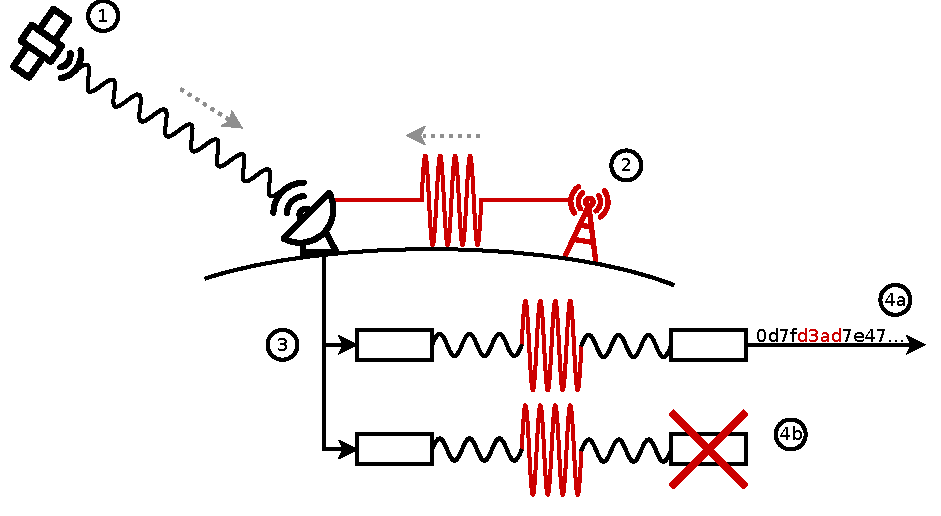
\includegraphics[width=\columnwidth]{diagrams/attack_illustration.pdf}
    \caption{An illustration of the attacks described in this paper. The attacker is indicated in red. 1)~The satellite broadcasts a signal; 2)~A ground-based attacker injects a crafted signal, overshadowing the legitimate signal and resulting in one of two scenarios; 3a)~The victim receiver decodes the attacker-controlled data, poisoning derived datasets; 3b)~The injected signal exploits vulnerabilities in the protocol decoders, resulting in denial of service or arbitrary code execution.}
    \label{fig:attack-illustration}
\end{figure}

% TODO: insert diagram of common space comms protocols
% TODO: find out which other satellites are unencrypted, and especially those which are new and use CCSDS
% Are they generally encrypted above the CCSDS layer?

\begin{figure}
    \centering
    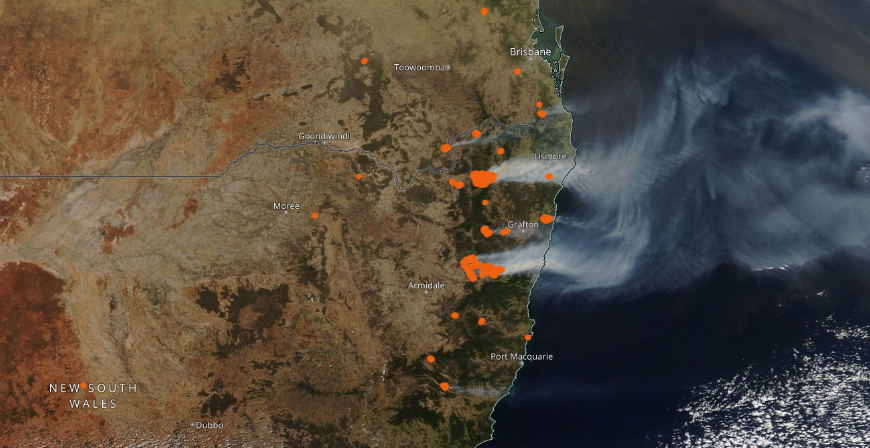
\includegraphics[width=\columnwidth]{diagrams/bushfire.png}
    \caption{The 2019 Australia bushfires as seen from Aqua's MODIS instrument, annotated with the \textit{Fires and Thermal Anomalies} dataset on NASA's worldview.\protect\footnotemark}
    \label{fig:bushfire}
\end{figure}

\footnotetext{Image taken from \url{https://worldview.earthdata.nasa.gov/?v=138.5214305912576,-37.663755528187544,165.90196079866635,-23.47436617591061\&as=2019-09-07-T00\%3A00\%3A00Z\&ae=2019-10-26-T16\%3A00\%3A00Z\&l=MODIS\_Combined\_Thermal\_Anomalies\_All,VIIRS\_SNPP\_Thermal\_Anomalies\_375m\_Day(hidden),VIIRS\_SNPP\_Thermal\_Anomalies\_375m\_Night(hidden),Reference\_Labels\_15m,Reference\_Features\_15m,Coastlines\_15m,VIIRS\_SNPP\_CorrectedReflectance\_TrueColor(hidden),MODIS\_Aqua\_CorrectedReflectance\_TrueColor,MODIS\_Terra\_CorrectedReflectance\_TrueColor(hidden)\&lg=false\&al=true\&av=3.5\&ab=on\&t=2019-09-07-T02\%3A00\%3A00Z}}


\begin{table*}
    \resizebox{\textwidth}{!}{%
    \begin{tabular}{lllll}
        \toprule
                     &       & \multicolumn{2}{c}{Satellites} & \\
        \cmidrule(lr){3-4}
        Organization & Usage & Provider & Nature & Data Access \\
        \midrule
        Planet Labs~\cite{planetProducts} & Various (intelligence, infrastructure, & Planet Labs & Self-operated & Commercial \\
                    & land use, water use) & & & \\
        Global Forest Watch~\cite{gfwMap} & Forest monitoring, carbon use, deforestation & Planet Labs & Commercial & Open access \\
        California Forest Observatory~\cite{cfoMap} & Monitoring forest fires in California & Planet Labs & Commercial & Open access \\
        ESRI~\cite{esriMap} & Land-use and land-cover maps & ESA (Sentinel-2) & Open access & Open access \\
        %Salo Sciences (TODO only bring back if I can say something about "forest restoration monitoring" project) & Conservation, climate monitoring & Planet Labs & Commercial & \\
        Meta~\cite{metaMap} & Population density maps & DigitalGlobe & Commercial & Open access \\
        Cloud to Street~\cite{cloudToStreet} & Flood tracking (disasters and insurance) & NASA (Terra/Aqua) & Open access & Commercial \\
        NCX Basemap~\cite{ncxBasemap} & Timber and carbon value monitoring in the USA & NASA & Open access & Commercial \\
        Upstream Tech HydroForecast~\cite{hydroforecast} & Water flow and weather intelligence & NASA (Terra/Aqua) & Open access & Commercial \\
        NASA FIRMS~\cite{nasaFirms} & Fire detection and management & NASA (EOS) & Self-operated & Open access \\
        \bottomrule
    \end{tabular}
    }
    \caption{Information on a number of satellite-derived datasets, including the satellite providers used to source the data.}
    \label{tab:satellite-derived-datasets}
\end{table*}
